\usetikzlibrary{positioning}
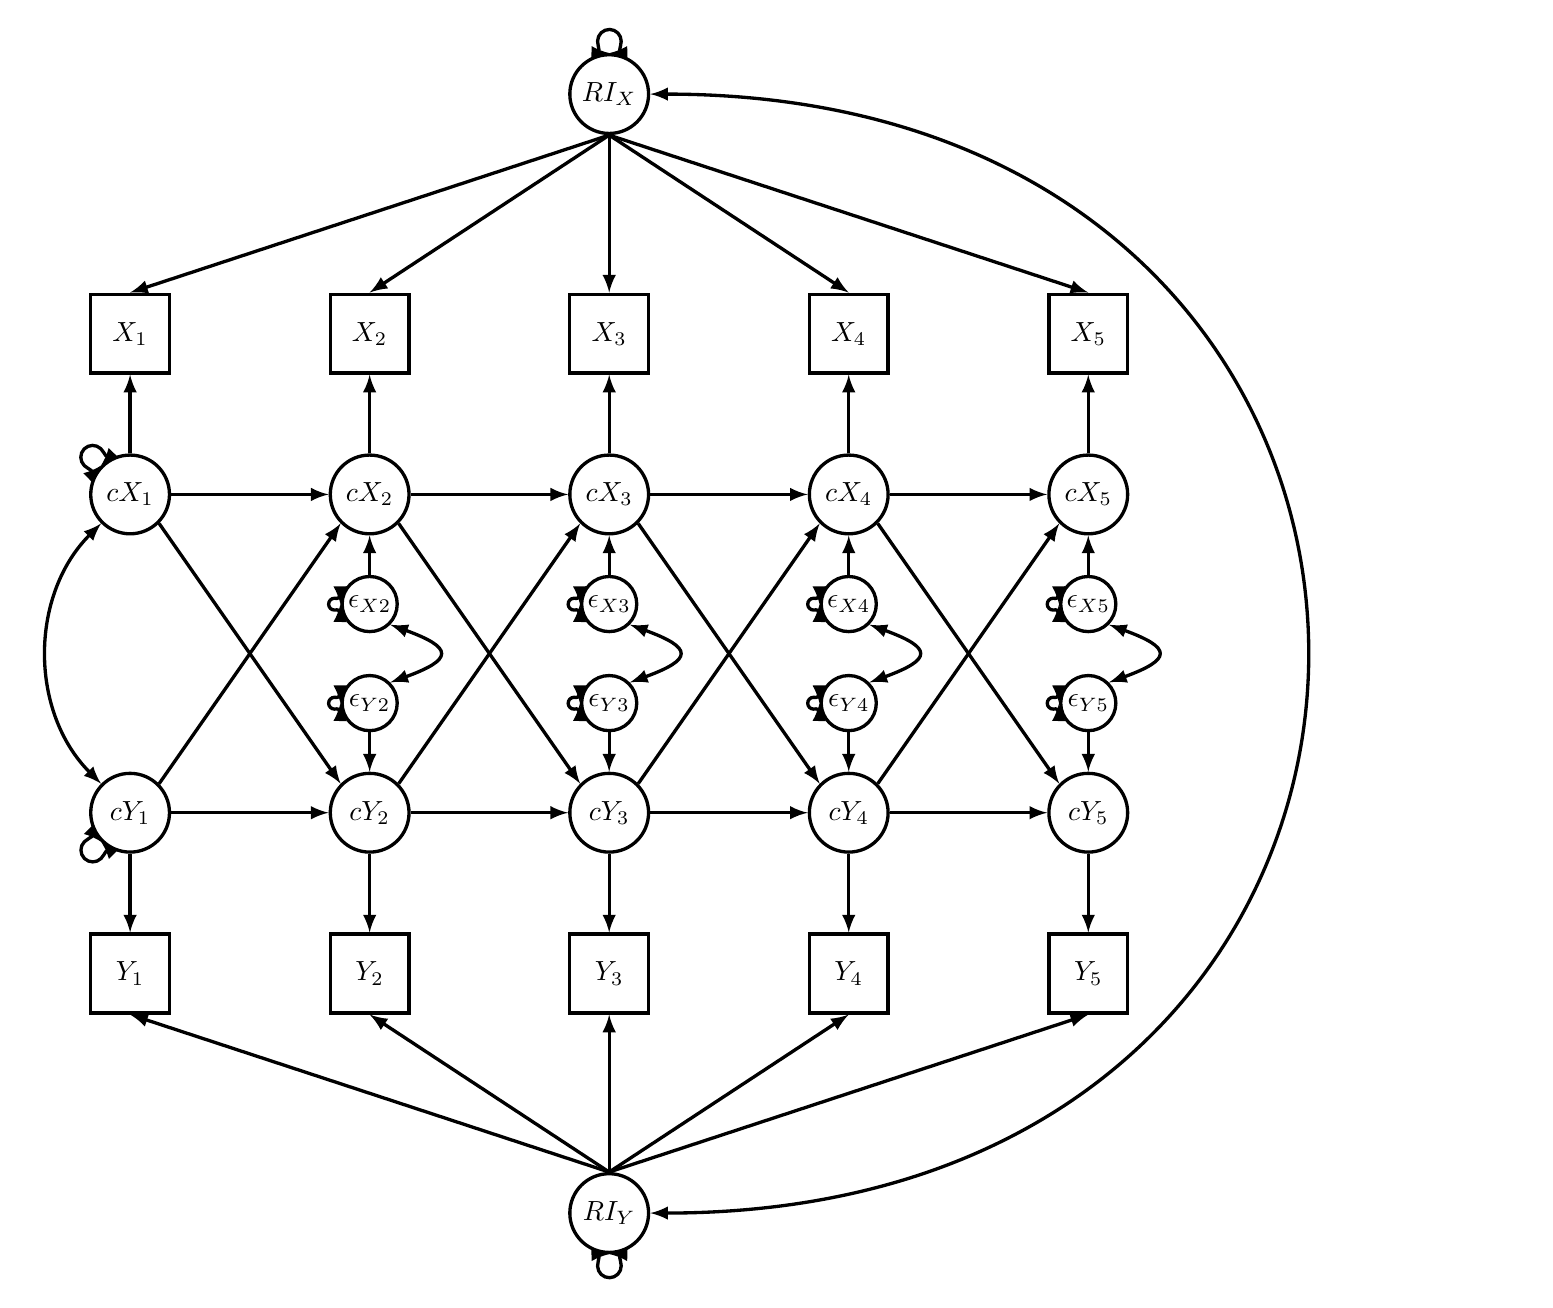
\begin{tikzpicture}[auto,node distance=.5cm, scale=0.5,
latent/.style={circle,draw,very thick,inner sep=0pt,minimum size=10mm,align=center},
manifest/.style={rectangle,draw,very thick,inner sep=0pt,minimum width=10mm,minimum height=10mm},
resid/.style={circle,draw,very thick,inner sep=0pt,minimum size=7mm,align=center},
paths/.style={->, very thick, -latex},
double/.style={very thick, latex-latex}
]
%create nodes
\node[latent] (cy1) at (0,0) {$cY_1$};
\node[latent, right=2cm of cy1] (cy2) {$cY_2$};
\node[latent, right=2cm of cy2] (cy3){$cY_3$};
\node[latent, right=2cm of cy3] (cy4){$cY_4$};
\node[latent, right=2cm of cy4] (cy5){$cY_5$};

\node[latent, above=3cm of cy1] (cx1){$cX_1$};
\node[latent, right=2cm of cx1] (cx2){$cX_2$};
\node[latent, right=2cm of cx2] (cx3){$cX_3$};
\node[latent, right=2cm of cx3] (cx4){$cX_4$};
\node[latent, right=2cm of cx4] (cx5){$cX_5$};

\node[resid, below=0.5cm of cx2] (ex2){$\epsilon_{X2}$};
\node[resid, below=0.5cm of cx3] (ex3){$\epsilon_{X3}$};
\node[resid, below=0.5cm of cx4] (ex4){$\epsilon_{X4}$};
\node[resid, below=0.5cm of cx5] (ex5){$\epsilon_{X5}$};

\node[resid, above=0.5cm of cy2] (ey2){$\epsilon_{Y2}$};
\node[resid, above=0.5cm of cy3] (ey3){$\epsilon_{Y3}$};
\node[resid, above=0.5cm of cy4] (ey4){$\epsilon_{Y4}$};
\node[resid, above=0.5cm of cy5] (ey5){$\epsilon_{Y5}$};

\node[manifest, above=1cm of cx1] (x1){$X_1$};
\node[manifest, above=1cm of cx2] (x2){$X_2$};
\node[manifest, above=1cm of cx3] (x3){$X_3$};
\node[manifest, above=1cm of cx4] (x4){$X_4$};
\node[manifest, above=1cm of cx5] (x5){$X_5$};

\node[manifest, below=1cm of cy1] (y1){$Y_1$};
\node[manifest, below=1cm of cy2] (y2){$Y_2$};
\node[manifest, below=1cm of cy3] (y3){$Y_3$};
\node[manifest, below=1cm of cy4] (y4){$Y_4$};
\node[manifest, below=1cm of cy5] (y5){$Y_5$};

\node[latent, above=2cm of x3] (etax){$RI_X$};
\node[latent, below=2cm of y3] (etay){$RI_Y$};

%observed to within paths
\draw[paths] (cx1) -- (x1);
\draw[paths] (cx2) -- (x2);
\draw[paths] (cx3) -- (x3);
\draw[paths] (cx4) -- (x4);
\draw[paths] (cx5) -- (x5);
\draw[paths] (cy1) -- (y1);
\draw[paths] (cy2) -- (y2);
\draw[paths] (cy3) -- (y3);
\draw[paths] (cy4) -- (y4);
\draw[paths] (cy5) -- (y5);

%draw paths

\draw[paths] (ex2) -- (cx2);
\draw[paths] (ex3) -- (cx3);
\draw[paths] (ex4) -- (cx4);
\draw[paths] (ex5) -- (cx5);

\draw[paths] (ey2) -- (cy2);
\draw[paths] (ey3) -- (cy3);
\draw[paths] (ey4) -- (cy4);
\draw[paths] (ey5) -- (cy5);

\draw[paths] (cx1.south east) -- (cy2.north west);
\draw[paths] (cx2.south east) -- (cy3.north west);
\draw[paths] (cx3.south east) -- (cy4.north west);
\draw[paths] (cx4.south east) -- (cy5.north west);
\draw[paths] (cy1.north east) -- (cx2.south west);
\draw[paths] (cy2.north east) -- (cx3.south west);
\draw[paths] (cy3.north east) -- (cx4.south west);
\draw[paths] (cy4.north east) -- (cx5.south west);

\draw[paths] (cx1.east) -- (cx2.west);
\draw[paths] (cx2.east) -- (cx3.west);
\draw[paths] (cx3.east) -- (cx4.west);
\draw[paths] (cx4.east) -- (cx5.west);
\draw[paths] (cy1.east) -- (cy2.west);
\draw[paths] (cy2.east) -- (cy3.west);
\draw[paths] (cy3.east) -- (cy4.west);
\draw[paths] (cy4.east) -- (cy5.west);

\draw[paths] (etax.south) -- (x1.north);
\draw[paths] (etax.south) -- (x2.north);
\draw[paths] (etax.south) -- (x3.north);
\draw[paths] (etax.south) -- (x4.north);
\draw[paths] (etax.south) -- (x5.north);

\draw[paths] (etay.north) -- (y1.south);
\draw[paths] (etay.north) -- (y2.south);
\draw[paths] (etay.north) -- (y3.south);
\draw[paths] (etay.north) -- (y4.south);
\draw[paths] (etay.north) -- (y5.south);

%draw covariances of residuals
\draw[double] (ex2.south east) to [out=-20, in=20, looseness=3](ey2.north east);
\draw[double] (ex3.south east) to [out=-20, in=20, looseness=3](ey3.north east);
\draw[double] (ex4.south east) to [out=-20, in=20, looseness=3](ey4.north east);
\draw[double] (ex5.south east) to [out=-20, in=20, looseness=3](ey5.north east);

%covariance cX1 and cY1
\draw[double](cx1.south west) to [out=225, in=135] (cy1.north west);

%draw variance of latent factors
\draw[double] (etax.north) arc [start angle=269, end angle = -89, x radius = 0.3cm, y radius=0.3cm];
\draw[double] (etay.south) arc [start angle=-269, end angle = 89, x radius = 0.3cm, y radius=0.3cm];

%draw residual variances
\draw[double] (ex2.west) arc [start angle=1, end angle = 359, x radius = 0.15cm, y radius=0.15cm];
\draw[double] (ex3.west) arc [start angle=1, end angle = 359, x radius = 0.15cm, y radius=0.15cm];
\draw[double] (ex4.west) arc [start angle=1, end angle = 359, x radius = 0.15cm, y radius=0.15cm];
\draw[double] (ex5.west) arc [start angle=1, end angle = 359, x radius = 0.15cm, y radius=0.15cm];

\draw[double] (ey2.west) arc [start angle=1, end angle = 359, x radius = 0.15cm, y radius=0.15cm];
\draw[double] (ey3.west) arc [start angle=1, end angle = 359, x radius = 0.15cm, y radius=0.15cm];
\draw[double] (ey4.west) arc [start angle=1, end angle = 359, x radius = 0.15cm, y radius=0.15cm];
\draw[double] (ey5.west) arc [start angle=1, end angle = 359, x radius = 0.15cm, y radius=0.15cm];

%draw variance cx1 and cy1
\draw[double] (cx1.north west) arc [start angle=-44, end angle = 314, x radius = 0.3cm, y radius=0.3cm];
\draw[double] (cy1.south west) arc [start angle=45, end angle = 405, x radius = 0.3cm, y radius=0.3cm];

%covariance between latent factors
\draw[double] (etax.east) to [out=0, in=0, looseness=2] (etay.east);

\end{tikzpicture}